\section{Size Matters: a Theoretical Analysis}

One important phenomenon observed in the above section (see \eg Table \ref{table:cifar10} and Figure \ref{fig:ocpooling}), as well as in related publications \cite{coates2010analysis,coates2011icml}, is that feature dimension almost always plays a key role in the final classification performance. With higher dimensional features and a simple linear classifier, performance usually appear to be monotonically increasing, although higher dimensionality comes with higher computational costs. It is also noteworthy that with a rather simple coding scheme and dictionary learning, results were in most cases comparable to the widely used but more computationally expensive sparse coding technique \cite{coates2011icml}. Furthermore, even selecting random dictionaries yielded close to state-of-the-art results. Further work on this domain \cite{freitas} suggests that the encoding technique used is a proxy to solving sparse coding (but in a simple and faster fashion).

The fact that random dictionaries perform well when operating with large codebook sizes poses interesting questions such as how feature size affects performance. In addition, even though the size of the dictionary (or codebook) is important, the accuracy seems to saturate, which is a phenomenon that was empirically verified in many tasks, and for which we now give a theoretical interpretation by linking random dictionaries with \nystrom sampling. In this section, we explain in detail how the feature learning approach could be viewed as a \nystrom sampling scheme from a high-dimensional (potentially infinite dimensional) feature space, and then derive proper bounds to model the behavior we observe in the classification experiments. We will use slightly different notations from the previous section, as we will focus on mathematics that is not necessarily binded to specific coding or pooling operations.

\subsection{The \nystrom Sampling View}
\nystrom sampling has been proposed as an efficient way to approximate large PSD matrices (such as kernel matrices) by sampling columns of the matrix. Specifically, let $\bK$ be an $N\times N$ matrix, the \nystrom method defines an approximation as $\bK' = \bE\bW^{+}\bE^\top$, where $\bE$ is a $N\times c$ matrix with the $c$ columns randomly sampled from those of $\bK$, and $\bW$ is the square $c\times c$ matrix formed by picking the same $c$ columns and rows from $\bK$. Such a sampling perspective have been shown to be very effective in kernel machines \cite{zhang2008improved,cortes10,kumar2012sampling}.

We consider forming a dictionary by sampling our training set (although, as discussed below, better techniques exist that lead to further gains in performance). To encode a new data point $\bx \in \mathbb{R}^d$, we apply a (generally non-linear) coding function $\bc$ so that $\bc(\bx) \in \mathbb{R}^c$. The standard classification pipeline considers $\bc(\bx)$ as the new feature space, and typically uses a linear classifier on this space. In this section, we consider the threshold encoding function as in \cite{coates2011icml}, $\bc(\bx) = \max(0,\bx^\top\bD - \alpha)$, but the derivations are valid for other different coding schemes.

In the ideal case (infinite computation and memory), we encode each sample $\bx$ using the whole training set $\bX \in \mathbb{R}^{d \times N}$, which can be seen as the best local coding of the training set $\bX$, to the extent that overfitting is handled by the classification algorithm. In fact, larger dictionary sizes yield better performance assuming the linear classifier is well regularized, as it can be seen as a way to do manifold learning \cite{wang2010locality}. We define the new features in this high-dimensional coded space as $\bC = \max(0,\bX^\top\bX - \alpha)$, where the $i$-th row of $\bC$ corresponds to coding the $i$-th sample $\bc(\bx_i)$. The linear kernel function between samples $i$ and $j$ is $K(\bx_i,\bx_j) = \bc(\bx_i)^\top\bc(\bx_j)$. Thus, performing linear classification on the coded features effectively uses the kernel matrix $\bK = \bC\bC^\top$.

In the conventional context of \nystrom sampling for kernels, one randomly samples a subset of the columns of $\bK$ and then replaces the original matrix $\bK$ with a low-rank approximation $\hat{\bK}$. However, in our problem, naively applying \nystrom sampling to the matrix $\bK$ does not save any computation, as every column of $\bK$ requires to encode the corresponding feature with the large dictionary of all $N$ samples. However, if we approximate the matrix $\bC$ with \nystrom sampling to obtain $\bC' \approx \bC$, we would get an efficient approximation of the kernel matrix as $\bK' \approx \bK$:
\begin{align}
\bC' & = \bE \bW^{-1} \bE^\top, \text{ and}\\
\bK' & = \bC' \bC'^\top = \bE \bW^{-1} \bE^\top \bE \bW^{-1} \bE^\top = \bE \bLambda \bE^\top,
\end{align}
where the first equation comes from applying \nystrom sampling to $\bC$, $\bE$ is a random subsample of the columns of $\bC$, and $\bW$ the corresponding square matrix with the same random subsample of both columns and rows of $\bC$.

We note that in the traditional coding scheme proposed in \cite{coates2011icml},  if the dictionary is taken randomly then $\bK_{coding} = \bE \bE^\top$, and by applying \nystrom sampling to $\bC$ we obtain almost the same kernel, where the matrix $\bLambda$ acts as an additional Mahalanobis metric on the coded space.
%eWe found the matrix $\bLambda$ to be strongly diagonal (even more so if instead of sampling, one tries to minimize the similarity between dictionary elements (such as in K-means)).
Adding the term $\bLambda$ seemed to help in some cases, when the dictionary size is small (for example, in the CIFAR10 dataset, classification performance was improved by about $0.5\%$ when $c<500$.). We refer to the supplementary material to discuss the effect of $\bLambda$ and how to efficiently find it without explicitly computing the original $N\times N$ matrix. 
%The conceptual diagram of the \nystrom sampling view can be seen in Figure \ref{fig:concept}.

\subsection{Error Bounds on the Approximation}

Many existing analyses have computed bounds on the error made in estimating $\bC$ by $\bC'$ by sampling $c$ columns, such as \cite{talwalkar2010matrix,kumar2012sampling}, but not between $\bK = \bC\bC^\top$ and $\bK'=\bC'\bC'^\top$, which we aim to analyze in this section. The bound we start with is \cite{kumar2012sampling}:
\begin{equation}
\label{eqn:nyst_bound}
||\bC-\bC'||_F \leq ||\bC-\bC_k||_F + \epsilon \max(n\bC_{ii}),
\end{equation}
valid if $c \geq 64k/\epsilon^4$ ($c$ is the number of columns that we sample from $\bC$ to form $\bE$, i.e. the codebook size), where $k$ is the sufficient rank to estimate the structure of $\bC$, and $\bC_k$ is the optimal rank $k$ approximation (given by Singular Value Decomposition (SVD), which we cannot compute in practice). %Note that, if we assume that our training set can be explained by a manifold of a certain dimension $k$ (i.e. the first term in the right hand side of Eqn.\ (\ref{eqn:nyst_bound}) vanishes), then the error is proportional to $\epsilon$ times a constant (that is dataset dependent).

Fixing $k$ to the value that retains enough energy from $\bC$, we get a bound that gives a minimum $\epsilon$ to plug in Eqn.\ \ref{eqn:nyst_bound} for every $c$ (sample dictionary size). This gives us a useful bound of the form $\epsilon \geq \hat{M}\left(\frac{1}{c}\right)^{\frac{1}{4}}$ for some constant $\hat{M}$ (that depends on $k$). Hence:
\begin{equation}
||\bC-\bC'||_F \leq O + M\left(\frac{1}{c}\right)^{\frac{1}{4}},
\end{equation}
where $O$ and $M$ constants that are dataset specific.

However, having bounded the error $\bC$ is not yet sufficient to establish how the code size will affect the classifier performance. In particular, it is not clear how the error on $\bC$ affect the error on the kernel matrix $\bK$. Similarly, having a kernel matrix of different quality will affect classification performance. Recent work \cite{cortes10} proves a linear relationship between kernel matrix degradation and classification accuracy. Furthermore, in the supplementary material, we provide a proof that shows the degradation of $\bK$ is also proportional to the degradation of $\bC$. Hence, the error bound on $\bK'$ is of the same form as the one we obtained for $\bC$:
\begin{equation}
||\bK-\bK'||_F \leq O' + M'\left(\frac{1}{c}\right)^{\frac{1}{4}}.
\label{eqn:bound}
\end{equation}

We briefly prove the bound here. Recall that $\bK = \bC\bC^\top$ and $\bK' = \bC'\bC'^\top$, and since $\bC$ and $\bC'$ are symmetric, $\bK = \bC^2$ and $\bK' = \bC'^2$. Note that the Frobenius norm satisfies subadditivity and submultiplicativity properties \cite{meyer01}, i.e.,
\begin{align}
    ||A+B||_F & \leq ||A||_F+||B||_F\text{, and}\\
    ||AB||_F & \leq ||A||_F||B||_F.
\end{align}
Thus, we have
\begin{align}
||\bK - \bK'|| & = ||\bC^2 - \bC'^2|| \\
& = ||(\bC-\bC')\bC + \bC'(\bC-\bC')|| \nonumber\\
& \leq ||(\bC-\bC')\bC|| + ||\bC'(\bC-\bC')||\nonumber\\
& \leq ||(\bC-\bC')||||\bC|| + ||\bC'||||(\bC-\bC')||\nonumber\\
& \leq ||(\bC-\bC')||||\bC|| + ||\bC'-\bC||^2 +\nonumber\\
& \phantom{\leq} + ||\bC||||(\bC-\bC')||\nonumber\\
& = ||(\bC-\bC')||\left(||(\bC-\bC')|| + 2||\bC||\right)\nonumber\\
& = \mathcal{O}(||(\bC-\bC')||)\nonumber
\end{align}
where all the $||.||$ are the Frobenius norms, and where in the last line we assumed that $||(\bC-\bC')||$ is sufficiently small and $||\bC||$ is constant w.r.t. $c$.  Thus, we can expect that the approximation quality of $\bK'$ will be similar than $\bC'$, and we will further assume that the quality of the kernel approximation $\bK'$ will determine the accuracy of the final classifier, which we will also empirically show in the experiments.

We note that the bound above also applies to the case when further steps, such as pooling, is carried out after coding, provided that such steps produce output feature dimensions that have a one-to-one correspondence with the dictionary entries. Pooling over multiple spatial regions does not change the analysis as it could be deemed as concatenating multiple kernel matrices for the data.

\begin{figure}
    \centering
    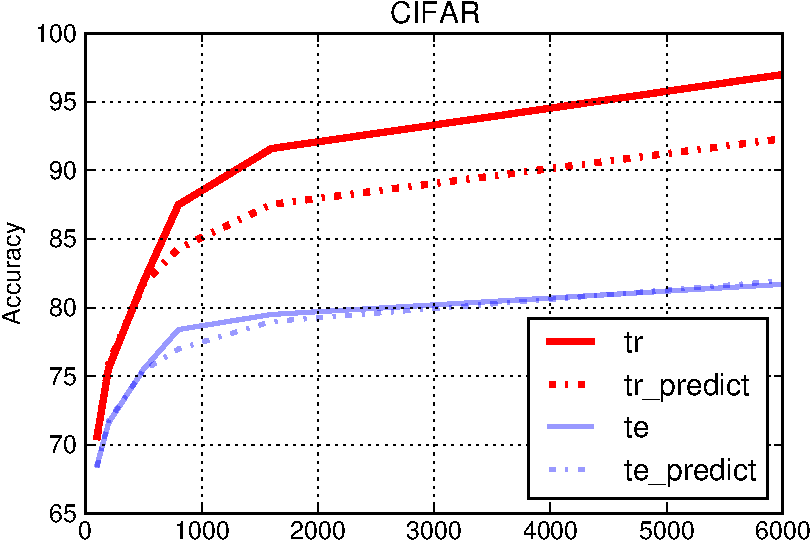
\includegraphics[width=0.4\textwidth]{figs/sizematters/bound_CIFAR.pdf}
    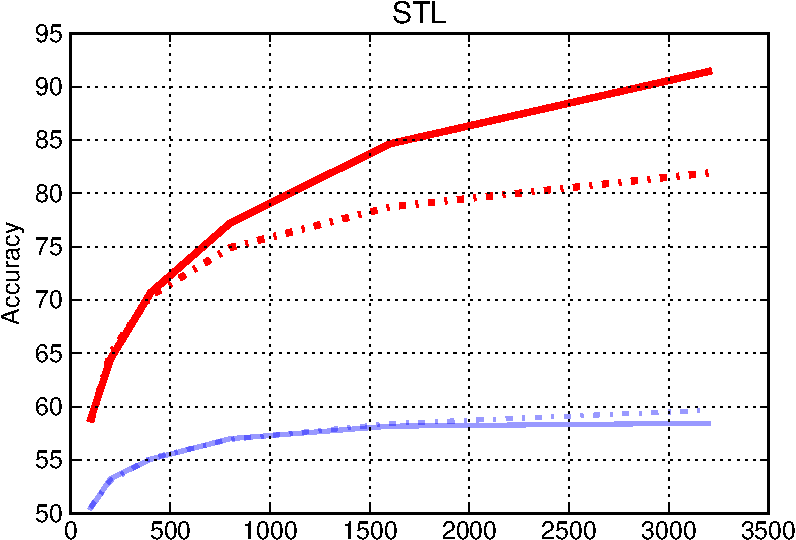
\includegraphics[width=0.4\textwidth]{figs/sizematters/bound_STL.pdf}
    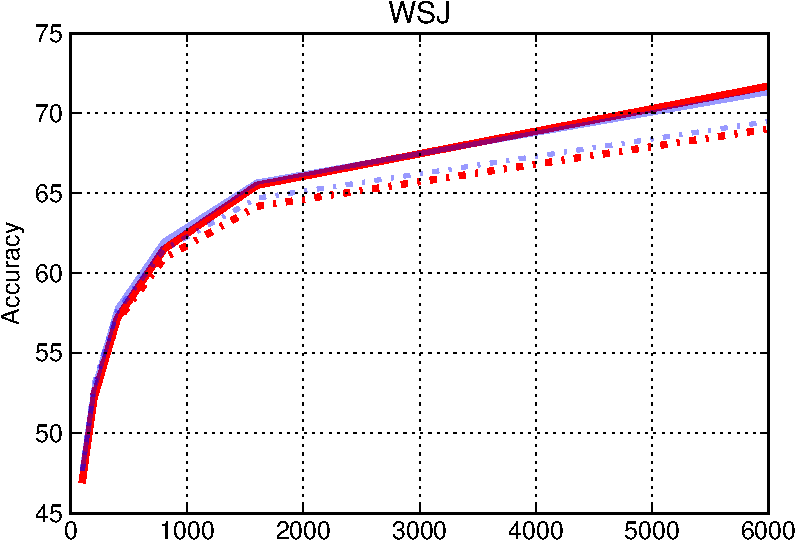
\includegraphics[width=0.4\textwidth]{figs/sizematters/bound_WSJ.pdf}
    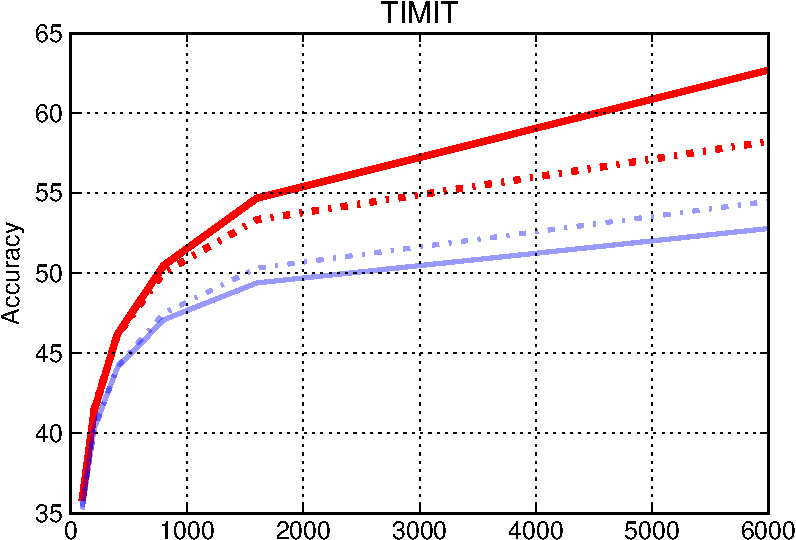
\includegraphics[width=0.4\textwidth]{figs/sizematters/bound_TIMIT.pdf}
    \caption{The actual training and testing accuracy (solid) and the predicted accuracy using our bound (dashed), on four datasets: CIFAR, STL, WSJ and TIMIT from left to right and top to bottom.}\label{fig:bounds}
\end{figure}

\subsection{Evaluating Bounds}
We empirically evaluate the bound on the kernel matrix, used as a proxy to model classification accuracy, which is the measure of interest. To estimate the constants in the bounds, we do interpolation of the observed accuracy using the first three samples of accuracy versus codebook size, which is of practical interest: one may want to quickly run a new dataset through the pipeline with small dictionary sizes, and then quickly estimate what the accuracy would be when running a full experiment with a much larger dictionary (which would take much longer to run) with our formulation. We always performed \nystrom sampling schemes by doing K-means instead of random selection (although the accuracy between both methods does not change too much when $c$ is sufficiently large).

In Figure \ref{fig:bounds} we plot the accuracy (on both train and test sets) on four datasets: CIFAR-10 and STL from vision, and WSJ and TIMIT from speech. For each dataset we used the first three samples to determine the constants given in the bound. One may practically favor this approach to evaluate performance, as small dictionary sizes are fast to try while large dictionary sizes are of interest. The bound is designed to predict training accuracy \cite{cortes10}, but we also do regression on testing accuracy for completeness. We note that testing accuracy will in general also be affected by the generalization gap, which is not captured by the bound analysis.

The results show that in all cases, the red dashed line is a lower bound of the training actual accuracy, and follows the shape of the empirical accuracy, predicting its saturation. In the testing case, our model is slightly optimistic when overfitting exists (e.g. STL and TIMIT), but correctly predicts the trend with respect to the number of dictionary entries.

The implication of linking \nystrom sampling theory to current learning pipelines has several immediate consequences: first, it clarifies why random sampling or K-means produce very reasonable dictionaries that are able to perform well in terms of classification accuracy \cite{zhang2008improved,coates2010aistats,kumar2012sampling}; more importantly, due to known bounds such as the one derived in this section, we can model how the codebook size will affect performance by running a few experiments with smaller codebook sizes, and extrapolating to larger (and more computationally expensive to compute) codebook sizes by means of Eq.~\ref{eqn:bound}, thus predicting accuracies before running potentially long jobs.

We further note that, although our experiment is carried out only by varying the number of codes in the dictionary (to better align speech and vision benchmarks), the pooling operation also falls under the same category: essentially, the whole coding + pooling pipeline could be viewed as a \nystrom sampling approach that samples features from the cartesian space of individial codes and individual pooling regions. Also, while we used the term ``sampling'', the actual feature selection does not necessarily have to be random: research in the \nystrom sampling methods suggests that more data-dependent feature selection approaches, notably K-means, works better than completely randomly sampling features \cite{zhang2008improved,kumar2012sampling}, while the theoretical bound still applies to these scenarios. Our work on selecting receptive fields aligns with such work, providing a more informed approach to find better pooled features for classification.

\section{PADL: Pooling Aware Dictionary Learning}\label{sec:sizematters:algorithm}

The \nystrom sampling view suggests that one could find a better subset of a large (potentially infinite) dictionary to obtain more informative features. In addition, existing work suggests that this could be often done in an efficient way with methods such as clustering. However, current clustering algorithms for dictionary learning \cite{coates2010aistats,coates2011icml} only apply to the local coding step, and do not consider the pooling effect. The \nystrom sampling insight suggests that simple feature selection approaches may exist that embraces more complex pipelines. As a concise example, we show that by explicitly taking into account the whole pipeline shown in Figure \ref{fig:pipeline} to include both local coding and pooling when learning the dictionary, one gets a much more compact feature representation.

Figure \ref{fig:feature_correlation} shows two examples why pooling-aware dictionary learning may be necessary, as local patch-based dictionary learning algorithms often yield similar filters with small translations. Such filters, even when uncorrelated on the patch level, produce highly correlated responses when pooled over a certain spatial region, leading to redundancy in the feature representation.

\begin{figure}
    \centering
    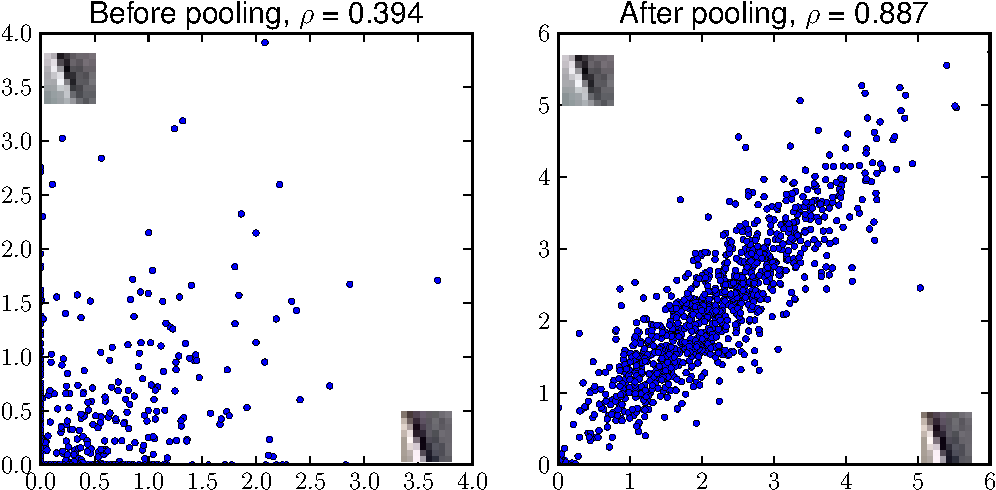
\includegraphics[width=0.7\linewidth]{figs/sizematters/distribution/12_distribution_final.pdf}\\
    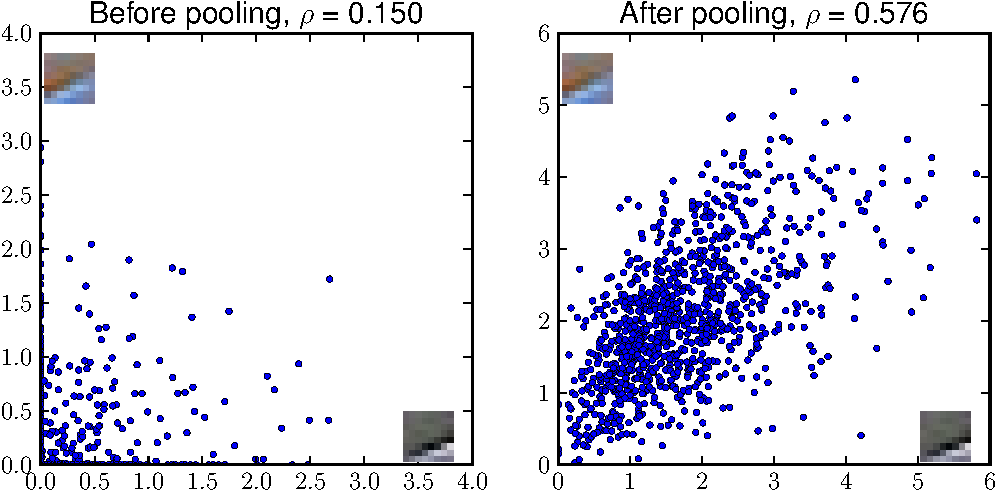
\includegraphics[width=0.7\linewidth]{figs/sizematters/distribution/34_distribution_final.pdf}
    \caption{Two codes learned from a patch-based K-means algorithm that produce lowly correlated patch-based responses (left), but highly correlated responses after pooling (right). Such phenomenon may root from various causes, such as codes with translational difference (above) and color difference (below).}\label{fig:feature_correlation}
\end{figure}

Observing the effectiveness of clustering methods in patch-based dictionary learning, we propose to learn a final dictionary of size $K$ in two stages: first, we adopt the K-means algorithm to learn a more over-complete starting dictionary of size $M$ ($M >> c$) on patches, effectively ``overshooting'' the dictionary we aim to obtain. We then perform encoding and pooling using the dictionary, and learn the final smaller dictionary of size $c$ from the statistics of the $M$-dimensional pooled features.

\subsection{Post-Pooling Feature Selection}
The first step of our algorithm is identical to the patch-based K-means algorithm with a dictionary size $M$. After this, we can sample a set of image super-patches of the same size as the pooling regions, and obtain the $M$ dimensional pooled features from them. Randomly sampling a large number of pooled features in this way allows us to analyze the pairwise similarities between the codes in the starting dictionary in a post-pooling fashion. We would then like to find a $c$-dimensional, lower dimensional subspace that best represents the $M$ pooled features.

If we simply would like to find a low-dimensional representation from the $M$-dimensional pooled features, one would naturally choose SVD to find the $K$ most significant projections of the covariance matrix. With a little abuse of terminology and denoting the matrix of randomly selected pooled feature as $\bX$ where each column is a feature vector, the SVD is carried out as
\begin{equation}
    \bX \approx \bU_c\bLambda_c\bV_c^\top,
\end{equation}
where $\bR$ is the covariance matrix computed using the random sample of pooled features, the $M\times c$ matrix $U_c$ contains the left singular vectors, and the $c\times c$ diagonal matrix $\bLambda_c$ contains the corresponding singular values. The low-dimensional features are then computed as $\bx_c = \bU_c^\top\bx$.

While the ``oracle'' low-dimensional representation by SVD guarantees the best $c$-dimensional approximation, it does not meet our goal since the dictionary size is not reduced, as SVD almost always yields non-zero coefficients for all the dimensions. Linearly combining the dictionary entries does not work either due to the nonlinear nature of the encoding algorithm. In our case, we would need the coefficients of only a subset of the features to be non-zero, so that a minimum number of filters need to be applied during testing time. Various machine learning algorithms aim to solve this, most notably structured sparse PCA \cite{jenatton2010structured}. However, these methods often requires a structured sparsity term to be applied during learning, making the training time-consuming and difficult to scale up.

Based on the analysis of the last section, the problem above could again be viewed as a \nystrom sampling problem by subsampling the rows of the matrix $\bX$ (corresponding to selecting codes from the large dictionary). Empirical results from the \nystrom sampling then suggests the use of clustering algorithms to solve this. Thus, we resort to a simpler K-centroids method.

Specifically, we use affinity propagation \cite{frey2007clustering}, which is a version of the K-centroids algorithm, to select exemplars from the existing dictionary. Intuitively, codes that produce redundant pooled output (such as translated versions of the same code) would have high similarity between them, and only one exemplar would be chosen by the algorithm. We briefly explain the affinity propagation procedure here: it finds exemplars from a set of candidates where pairwise similarity $s(i,j)$ ($1 \leq i, j \leq M$) can be computed. It iteratively updates two terms, the ``responsibility'' $r(i,j)$ and the ``availability'' $a(i,j)$ via a message passing method following such rules \cite{frey2007clustering}:
\begin{align}
    r(i,k) & \leftarrow s(i,k) - \max_{k'\neq k}\{a(i,k') + s(i,k')\}\label{ap:r}\\
    a(i,k) & \leftarrow \min\{0, r(k,k) + \sum\nolimits_{i'\notin\{i,k\}}\max\{0, r(i',k)\}\}\nonumber\\
           & \phantom{\leftarrow } (\text{if } i \neq k)\\
    a(k,k) & \leftarrow \sum\nolimits_{i'\neq k} \max\{0, r(i', k)\}\label{ap:a}
\end{align}
Upon convergence, the centroid that represents any candidate $i$ is given by $\arg\max_{k} (a(i,k) + r(i,k))$, and the set of centroids $\mathcal{S}$ is obtained by
\begin{equation}
    \mathcal{S} = \{k | \exists i,k \text{ s.t. } k = \arg\max_{k'} (a(i,k') + r(i,k'))\}
\end{equation}
And we refer to \cite{frey2007clustering} for details about the nature of such message passing algorithms. The similarity between two pooled dimensions (which correspond to two codes in the starting dictionary) $i$ and code $j$, as in Eqn.\ (\ref{ap:r})-(\ref{ap:a}), is computed as
\begin{equation}
    s(i,j) = \frac{2R_{ij}}{\sqrt{R_{ii}R_{jj}}} - 2.
\end{equation}
Note that this is equivalent to the negative Euclidean distance between the coded output $i$ and the coded output $j$ when the outputs are normalized to have zero mean and standard deviation 1. We note that related work such as \cite{coates2012emergence} adopt a similar approach by max-pooling the outputs of similar codes to generate next-layer features in a deep fashion. Our method shares the same merit while focusing on model compression by bounding the computation time in a single layer.

Clustering algorithms has shown to be very effective in the context of \nystrom sampling \cite{kumar2012sampling}, and are often highly parallelizeable, easily being scaled up by simply distributing the data over multiple machines. This allows us to maintain the efficiency of dictionary learning. Using a large, overshooting starting dictionary allows us to preserve most information from the patch-level, and the second step prunes away the redundancy due to pooling. Note that the large dictionary is only used during the feature learning time - after this, for each input image, we only need to encode local patches with the selected, relatively smaller dictionary of size $c$, not any more expensive than existing feature extraction methods.



\section{Experiments for PADL}\label{sec:sizematters:experiments}
In this section we empirically evaluate two sets of experiments: using the bound to approximate the classification accuracy, and using the two-staged clustering algorithm to find better pooling invariant dictionaries.
%We apply our pooling-invariant dictionary learning (PADL) algorithm on several benchmark tasks, including the CIFAR-10 and STL datasets on which performance can be systematically analyzed, and the fine-grained classification task of classifying bird species, on which we show that feature learning provides a significant performance gain compared to conventional methods.

\begin{figure}[t]
    \centering
        \newcommand{\codeheight}{0.25}
        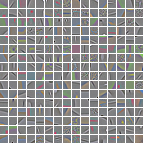
\includegraphics[height=\codeheight\linewidth]{figs/sizematters/centroids/dictionary_ap.png}\qquad\qquad
        
\includegraphics[height=\codeheight\textwidth]{figs/sizematters/centroids/1-neighbors.png}
        
\includegraphics[height=\codeheight\textwidth]{figs/sizematters/centroids/2-neighbors.png}
        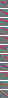
\includegraphics[height=\codeheight\textwidth]{figs/sizematters/centroids/6-neighbors.png}
        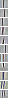
\includegraphics[height=\codeheight\textwidth]{figs/sizematters/centroids/89-neighbors.png}
        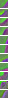
\includegraphics[height=\codeheight\textwidth]{figs/sizematters/centroids/42-neighbors.png}
        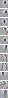
\includegraphics[height=\codeheight\textwidth]{figs/sizematters/centroids/38-neighbors.png}
        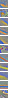
\includegraphics[height=\codeheight\textwidth]{figs/sizematters/centroids/44-neighbors.png}
        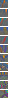
\includegraphics[height=\codeheight\textwidth]{figs/sizematters/centroids/110-neighbors.png}
        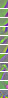
\includegraphics[height=\codeheight\textwidth]{figs/sizematters/centroids/156-neighbors.png}
        
\includegraphics[height=\codeheight\textwidth]{figs/sizematters/centroids/160-neighbors.png}
        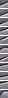
\includegraphics[height=\codeheight\textwidth]{figs/sizematters/centroids/162-neighbors.png}
        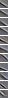
\includegraphics[height=\codeheight\textwidth]{figs/sizematters/centroids/200-neighbors.png}
        
\includegraphics[height=\codeheight\textwidth]{figs/sizematters/centroids/205-neighbors.png}
        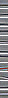
\includegraphics[height=\codeheight\textwidth]{figs/sizematters/centroids/212-neighbors.png}
        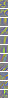
\includegraphics[height=\codeheight\textwidth]{figs/sizematters/centroids/216-neighbors.png}
        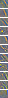
\includegraphics[height=\codeheight\textwidth]{figs/sizematters/centroids/222-neighbors.png}
        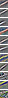
\includegraphics[height=\codeheight\textwidth]{figs/sizematters/centroids/229-neighbors.png}
    \caption{Visualization of the learned codes. Left: the selected subset of 256 centroids from an original set of 3200 codes. Right: The similarity between each centroid and the other codes in its cluster. For each column, the first code is the selected centroid, and the remaining codes are in the same cluster represented by it. Notice that while translational invariance is the most dominant factor, our algorithm does find invariances beyond that (e.g., notice the different colors on the last column). Best viewed in color.}\label{fig:centroidcodes}
\end{figure}

\begin{figure}
    \centering
    \begin{tabular}{ccc}
        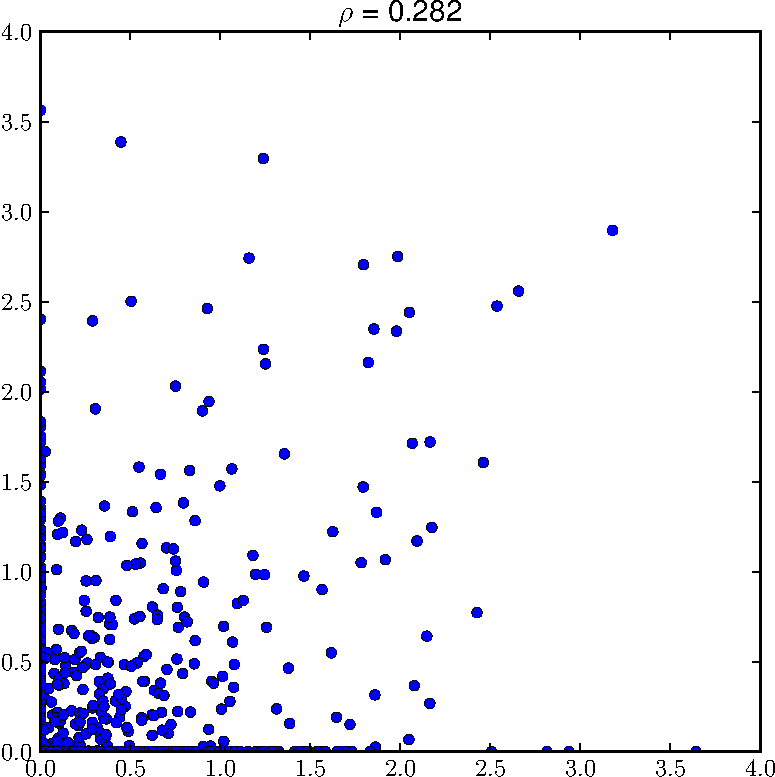
\includegraphics[height=0.25\textwidth]{figs/sizematters/distribution/within_cluster_prepooling.pdf} &
        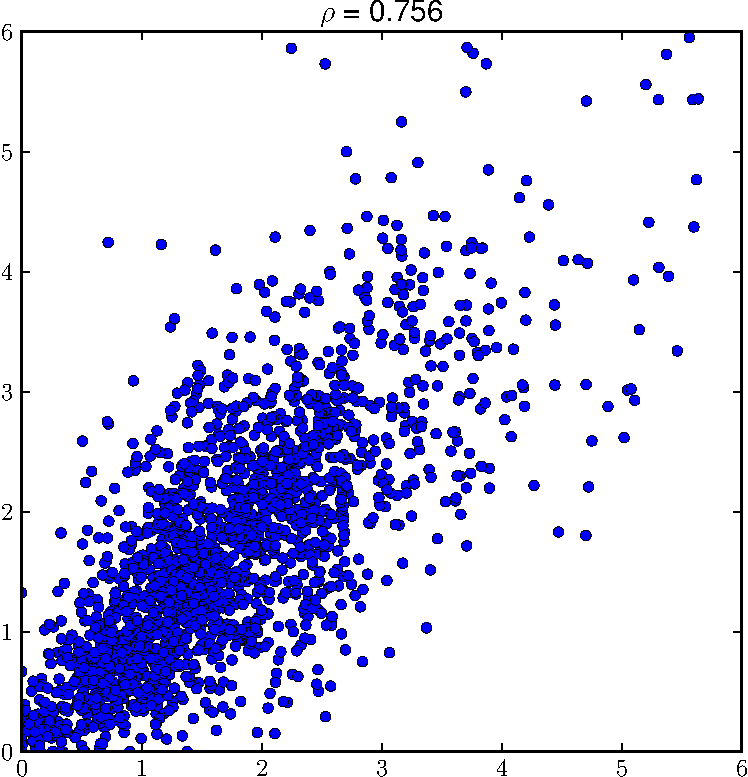
\includegraphics[height=0.25\textwidth]{figs/sizematters/distribution/within_cluster_postpooling.pdf} &
        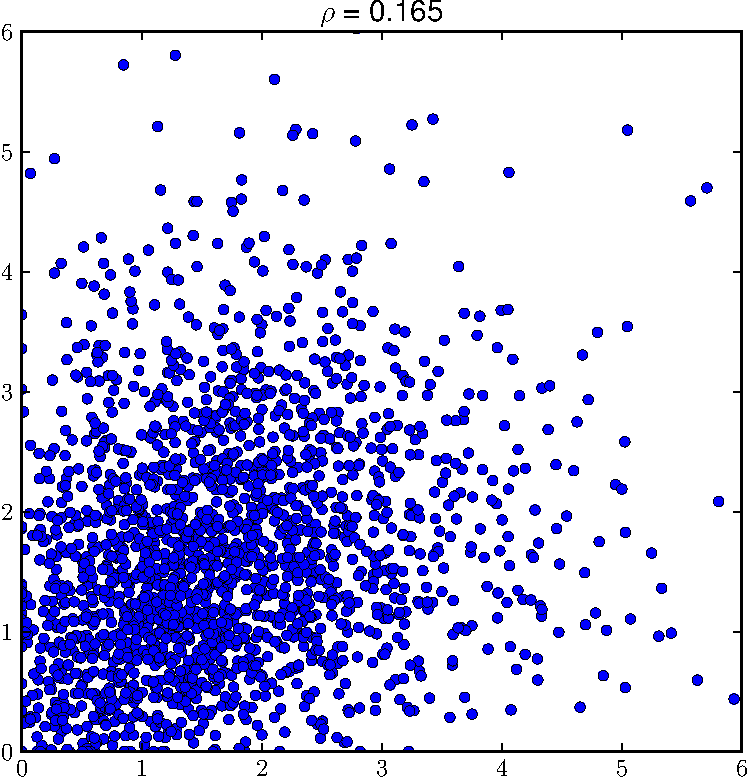
\includegraphics[height=0.25\textwidth]{figs/sizematters/distribution/between_centroids_postpooling.pdf}\\
        (a) & (b) & (c)
    \end{tabular}\\
    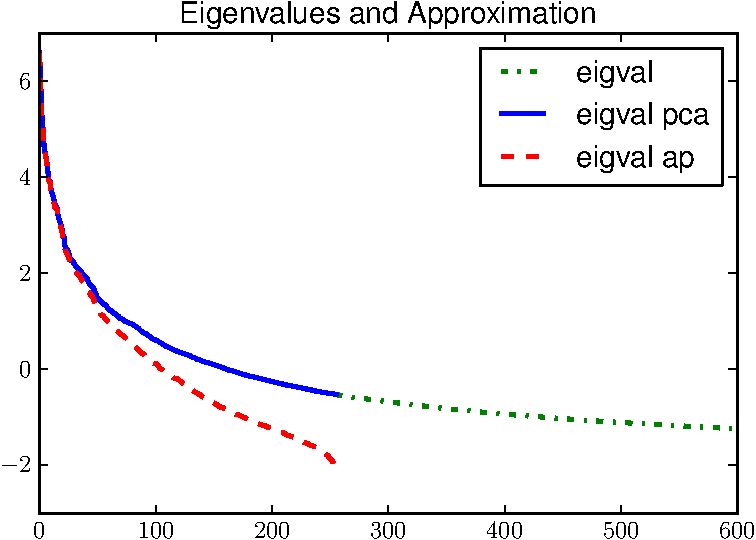
\includegraphics[height=0.3\textwidth]{figs/sizematters/centroids/eigvals.pdf}\\
    (d)
    \caption{(a)-(c): The filter responses before and after pooling: (a) before pooling, between codes in the same cluster (correlation $\rho=0.282$), (b) after pooling, between codes in the same cluster ($\rho = 0.756$), and (c) after pooling, between the selected centroids ($\rho = 0.165$), (d): the eigenvalues of the approximated matrix (in log scale).}\label{fig:pairwiseresponses}
\end{figure}

\subsection{Analysis of Selected Filters}\label{subsec:sizematters:visualization}
To visually show what codes are selected by affinity propagation, we applied our approach to the CIFAR-10 dataset by first training an over-complete dictionary of 3200 codes following \cite{coates2011icml}, and then performing affinity propagation on the 3200-dimensional pooled features to obtain 256 centroids, which we visualize in Figure \ref{fig:centroidcodes}. Translational invariance appears to be the most dominant factor, as many clusters contain translated versions of the same Gabor like code, especially for gray scale codes. On the other hand, clusters capture more than translation: clusters such as column 5 focus on finding the contrasting colors more than finding edges of exactly the same angle, and clusters such as the last column finds invariant edges of varied color. We note that the selected codes are not necessarily centered, as the centroids are selected solely from the pooled response covariance statistics, which does not explicitly favor centered patches.

We could also verify whether the second clustering stage captures the pooling invariance by checking the statistics of three types of filter responses: (a) pairwise filter responses \emph{before pooling} between codes in the same cluster, (b) pairwise filter responses \emph{after pooling} between codes in the same cluster, and (c) pairwise filter responses after pooling between the selected centroids. The distribution of such responses shown in Figure \ref{fig:pairwiseresponses} verifies our argument: first, codes that produce uncorrelated responses before pooling may become correlated after the pooling stage (Figure \ref{fig:pairwiseresponses}(a,b)); second, by explicitly considering the pooled feature statistics, we are able to select a subset of the dictionary whose responses are lowly correlated (Figure \ref{fig:pairwiseresponses}(b,c)), preserving more information with a fixed number of codes. In addition, Figure \ref{fig:pairwiseresponses}(d) shows the eigenvalues of the original covariance matrix and those of the approximated matrix, showing that the approximation captures the largest eigenvalues of the original covariance matrix well.

\begin{table}
    \centering
    \begin{tabular}{ccc}
    \hline
    %\abovespace\belowspace
    Task & Learning Method & Accuracy\\
    \hline
    %\abovespace
                & K-means   & 69.02 \\
    CIFAR-10    & 2x PADL    & 70.54 (+1.52) \\
    200 codes   & 4x PADL    & 71.18 (+2.16) \\
    %\belowspace
                & 8x PADL    & 71.49 (+2.47) \\
    \hline
    %\abovespace
    CIFAR-10    & K-means   & 77.97 \\
    %\belowspace
    1600 codes  & 2x PADL    & 78.71 (+0.74) \\
    \hline
  \end{tabular}
  \caption{Classification Accuracy on the CIFAR-10 and STL datasets under different budgets.}\label{tab:cifarstl}
\end{table}

\begin{figure}[t]
    \centering
    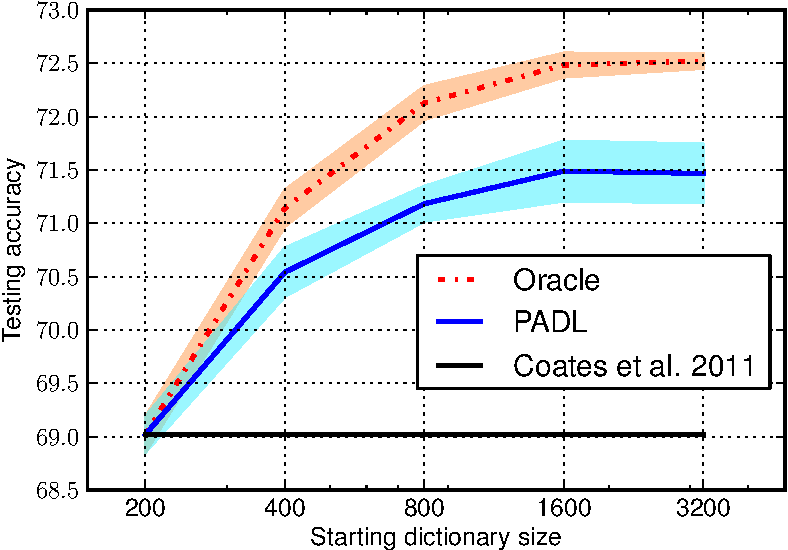
\includegraphics[width=0.5\textwidth]{figs/sizematters/cifar_improvement.pdf}
    \caption{Performance improvement on CIFAR when using different starting dictionary sizes and a final dictionary of size 200. Shaded areas denote the standard deviation over different runs. Note that the x-axis is in log scale.}\label{fig:relativeimprovement}
\end{figure}

\subsection{Pooling Invariant Dictionary Learning}\label{subsec:sizematters:exp:classification}
To evaluate the improvement introduced by learning a pooling invariant dictionary as in Section \ref{sec:sizematters:algorithm}, we show in Figure \ref{fig:relativeimprovement} the relative improvement obtained on CIFAR-10 when we use a fixed dictionary size 200, but perform feature selection from a larger overshooting dictionary as indicated by the X axis. The SVD performance is also included in the figure as an ``oracle'' for the feature selection performance. Learning the dictionary with our feature selection method consistently increases the performance as the size of the original dictionary increases, and is able to get about two thirds the performance gain as obtained by the oracle performance. We note again that SVD still requires the large dictionary to be used and does not save any testing time.

The detailed performance gain of our algorithm on the two datasets, using different overshooting and final dictionary sizes, is visualized in Figure \ref{fig:cifarstl}. Table \ref{tab:cifarstl} summarizes the accuracy values of two particular cases - final dictionary sizes of 200 and 1600 respectively, on CIFAR. Note that our goal is not to get the best overall performance - as performance always goes up when we use more codes. Rather, we focus on two evaluations: (1) how much gain we get given a fixed dictionary size as the budget, and (2) how much computation time we save to achieve the same accuracy.

Overall, considering the pooled feature statistics always help us to find better dictionaries, especially when relatively small dictionaries are used. During testing time, it costs only about 60\% computation time with PADL to achieve the same accuracy as K-means does. For the STL dataset, an overly large starting dictionary may lessen the performance gain (Figure \ref{fig:cifarstl}(b)) possibly due to feature selection being more prone to local optimum and the small number of training data (thus more overfitting). However, in general the codebook learned by PADL is consistently better than its patch-based counterpart, suggesting the applicability of the \nystrom sampling view in feature learning with a multi-layer structure including spatial pooling.

\begin{figure}
    \centering
    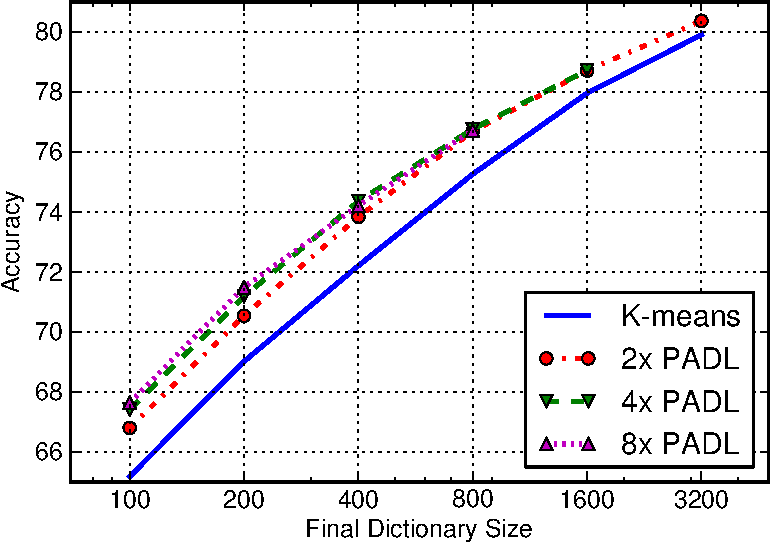
\includegraphics[width=0.4\textwidth]{figs/sizematters/cifar_accuracy.pdf}
    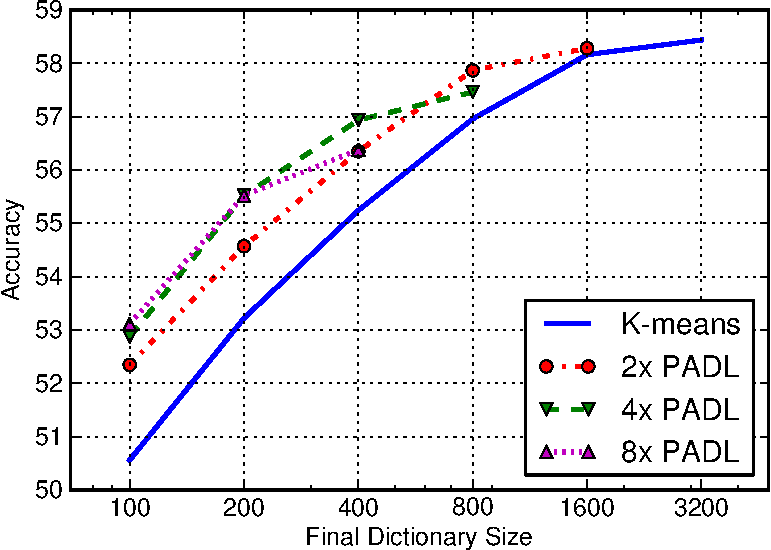
\includegraphics[width=0.4\textwidth]{figs/sizematters/stl_accuracy.pdf}\\
    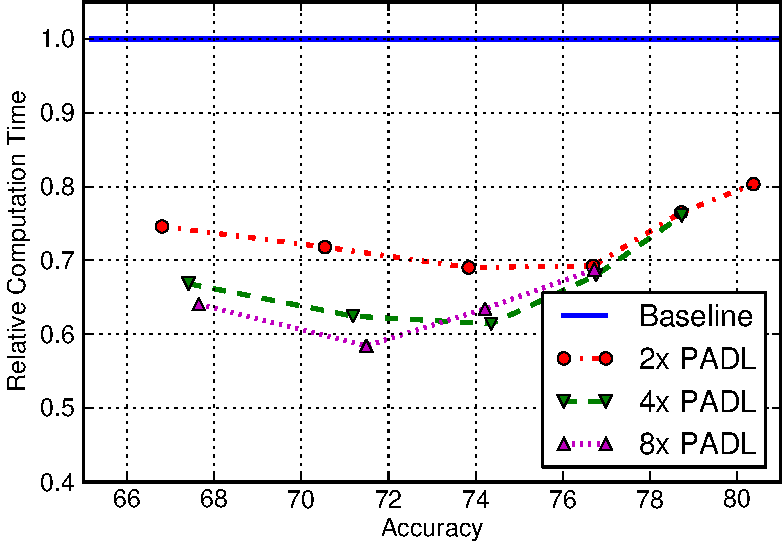
\includegraphics[width=0.4\textwidth]{figs/sizematters/cifar_speedup.pdf}
    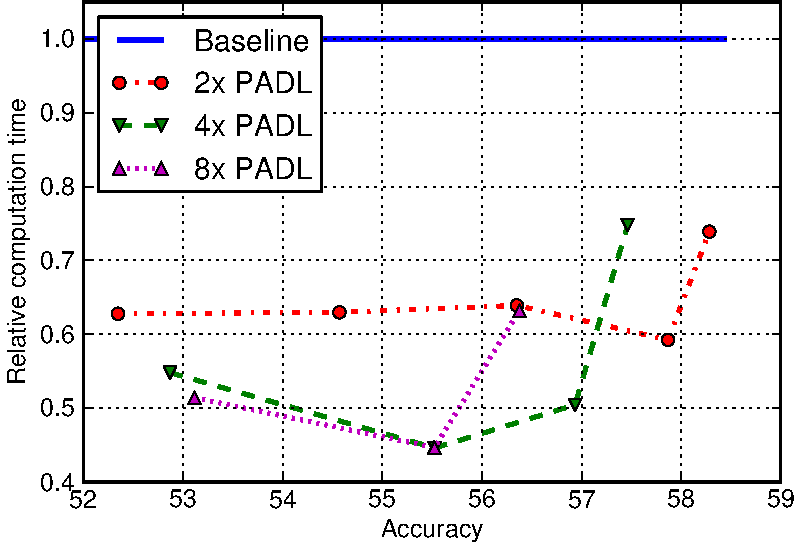
\includegraphics[width=0.4\textwidth]{figs/sizematters/stl_speedup.pdf}
    \caption{Above: accuracy values on the CIFAR-10 (left) and STL (right) datasets under different dictionary size budgets. ``nx PADL'' means learning the dictionary from a starting dictionary that is n times larger. Below: Relative computation time to achieve the same accuracy using dictionary obtained from PADL.}\label{fig:cifarstl}
\end{figure}

Finally, we note that due to the heavy-tailed nature of the encoded and pooled features (see the eigendecomposition of Figure \ref{fig:pairwiseresponses}), one can infer that the representations obtained with a budget would have a correspondingly bounded performance when combined with linear SVMs. We have focused on analyzing unsupervised approaches, but incorporating weakly supervised information to guide feature learning / selection or learning multiple layers of feature extraction would be particularly interesting, and would be a possible future direction.
